
\subsection{Information Layer}
%\addcontentsline{toc}{subsection}{Information Layer}
The Information Layer specifies the Information Model, the domain-agnostic, common language of the International Data Spaces. The Information Model is an essential agreement shared by the participants and components of the IDS, facilitating compatibility and interoperability. The primary purpose of this formal model is to enable (semi-)automated exchange of digital resources within a trusted ecosystem of distributed parties, while preserving data sovereignty of Data Owners. The Information Model therefore supports the description, publication and identification of data products and reusable data processing software (both referred to hereinafter as $``$Digital Resources$"$ , or simply $``$Resources$"$ ). Once the relevant Resources are identified, they can be exchanged and consumed via semantically annotated, easily discoverable services. Apart from those core commodities, the Information Model describes essential constituents of the International Data Spaces, its participants, its infrastructure components, and its processes.

\subsubsection{Scope}
%\addcontentsline{toc}{subsubsection}{Scope}
The Information Model is a generic model, with no commitment to any particular domain. Domain modeling is delegated to shared vocabularies and data schemata, as provided e.g. by domain-specific communities of the International Data Spaces. The Information Model does not provide a meta-model for defining custom datatypes comparable to standards such as OData\footnote{https://www.odata.org/ } or OPC-UA\footnote{https://opcfoundation.org/ }. Concerns beyond the scope of modeling Digital Resources and their interchange are considered out of scope. The Information Model therefore does not deal with the side effects of data exchange (e.g. in scenarios in which data is used for time-critical machine operations).

\subsubsection{Model Representations}
%\addcontentsline{toc}{subsubsection}{Model Representations}
The Information Model has been specified at three levels of formalization. Each level corresponds to a digital representation, ranging from this high-level, conceptual document down to the level of operational code, as depicted in Figure \ref{fig:Representations_of_the_Information_Model}. Every representation depicts the complete Information Model in its particular way. Among the different representations, the Declarative Representation (IDS Vocabulary) is the only normative specification of the Information Model. As such, it is accompanied by a set of auxiliary resources (e.g. guidance documents, reference examples, validation tools, and editing tools intended to support a competent, appropriate, and consistent usage of the IDS Vocabulary).


\paragraph{Conceptual Representation \\}
%\addcontentsline{toc}{paragraph}{Conceptual Representation }
The Conceptual Representation of the Information Model presents a high-level overview of the main, largely invariant concepts, with no commitment to a particular technology or domain. It targets a general audience, management boards, and media, as it provides basic information and promotes a shared understanding of the concepts by means of a textual document and a plausible visual notation. If available, references to related elements of the Declarative Representation and a Programmatic Representation are provided, encouraging the reader to take a look at these alternative implementations.

\paragraph{Declarative Representation\\}
%\addcontentsline{toc}{paragraph}{Declarative Representation}
The Declarative Representation (IDS Vocabulary) provides a normative view of the Information Model of the International Data Spaces.\footnote{https://github.com/IndustrialDataSpace/InformationModel }
%% ToDo: change to https://github.com/International-Data-Spaces-Association/InformationModel once repository has been moved.  (FIT still needs the permission to do so!)
It has been developed along the analysis, findings, and requirements of the Conceptual Representation. Based on a stack of W3C Semantic Web technology standards\footnote{https://www.w3.org/standards/semanticweb/ } and standard modeling vocabularies (DCAT\footnote{https://www.w3.org/TR/vocab-dcat-2/ }, ODRL\footnote{https://www.w3.org/TR/odrl-model/ }, SKOS\footnote{https://www.w3.org/TR/skos-reference/ }, etc.), it provides a formal, machine-interpretable specification of concepts envisaged by the Conceptual Representation, residing at the persistent namespace URI \url{https://w3id.org/idsa/core/}. Furthermore, it details and formally defines entities of the International Data Spaces in order to be able to share, search for, and reason upon the structured metadata describing these entities. As such, it comprises a complete referential model allowing the derivation of a number of Programmatic Representations. The IDS Vocabulary is typically used and instantiated by knowledge engineers, ontology experts, or information architects. It defines a fairly minimal, domain-agnostic $``$core model$"$  and relies on third-party standard and custom vocabularies in order to express domain-specific facts. According to the common practice, existing domain vocabularies and standards are reused where possible, fostering acceptance and interoperability.


\paragraph{Programmatic Representation\\}
%\addcontentsline{toc}{paragraph}{Programmatic Representation}
The Programmatic Representation of the Information Model targets Software Providers by supporting seamless integration of the Information Model with a development infrastructure software developers are familiar with. It comprises a programming language data model (e.g., Java, Python, C++) shipped as a set of documented software libraries (e.g., JAR files).\footnote{https://github.com/International-Data-Spaces-Association/IDS-G/blob/master/repositories/README.md }
% ToDo: IDS-G should provide the single point of truth.  @Sebastian Steinbuß, this is the most specific link I can imagine.  However, that page does not have an easy-to-spot section "programmatic representation of the infomodel", but one has to search in order to find out that "Artifactory, Fraunhofer IAIS" provides the desired information, and this link could also still be improved (https://github.com/International-Data-Spaces-Association/IDS-G/issues/2).
The Programmatic Representation provides a best-effort mapping of the IDS Vocabulary onto native structures of a target programming language. This approach supports type-safe development, well-established unit testing, and quality assurance processes. It allows developers to easily create instances of the Information Model that are compliant with the IDS Vocabulary, relieving them from the intricacies of ontology processing.



%%%%%%%%%%%%%%%%%%%% Figure/Image No: 22 starts here %%%%%%%%%%%%%%%%%%%%

\begin{figure}[H]
	\begin{Center}
		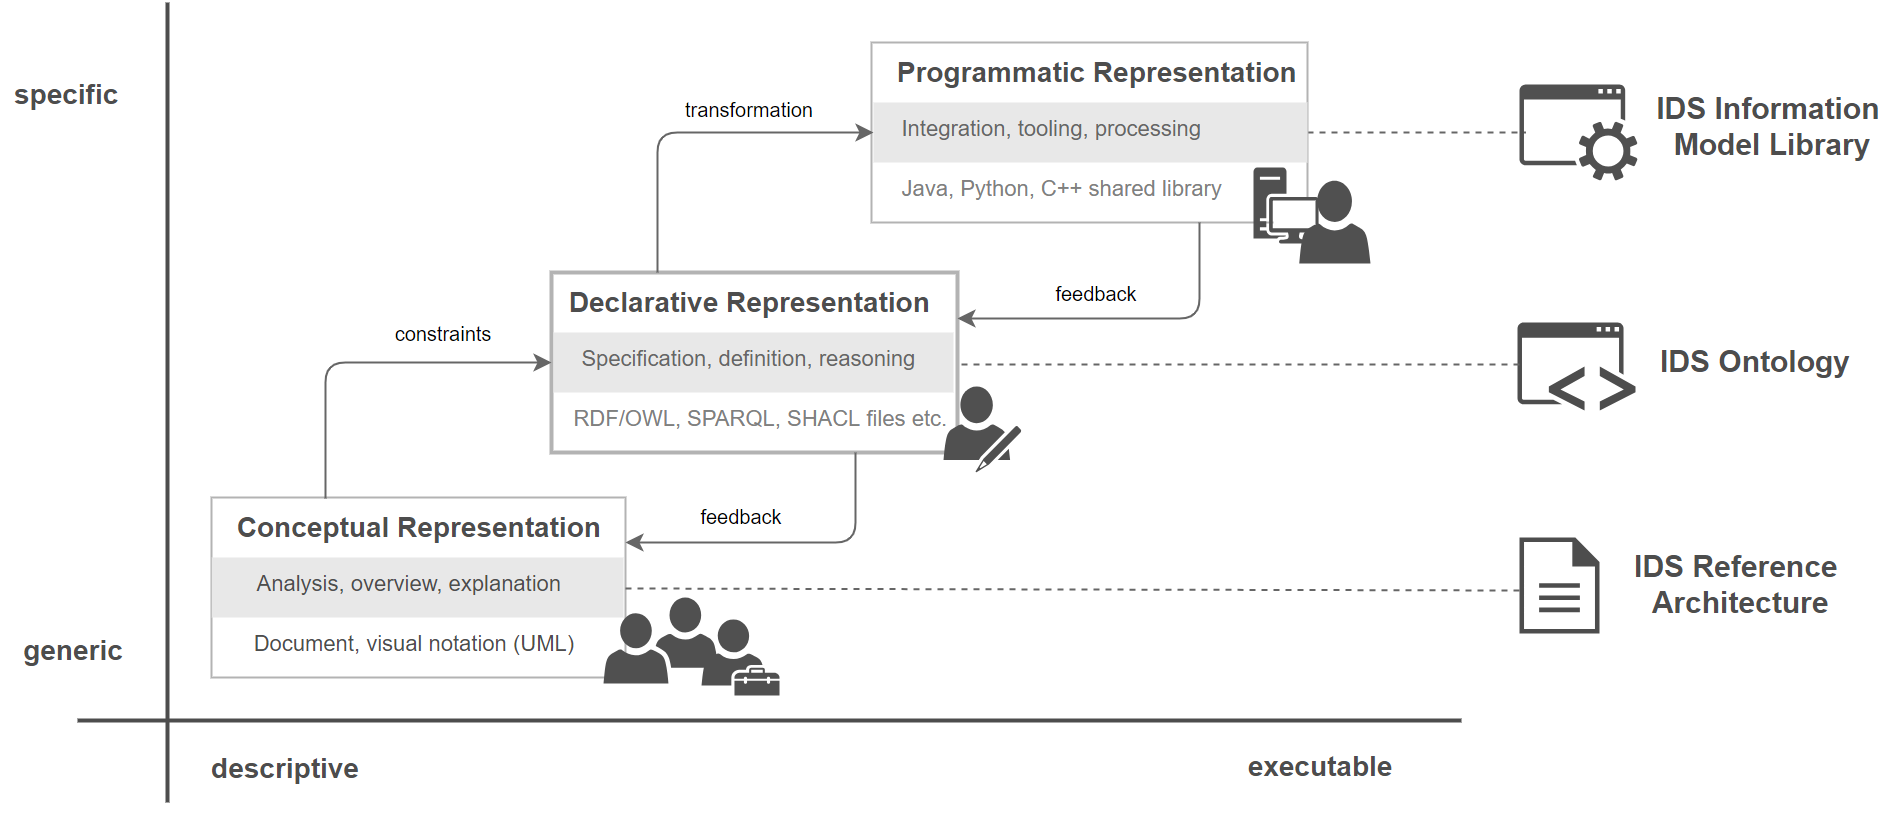
\includegraphics[width=6.53in,height=2.83in]{./media/image31.png}
		\caption{Representations of the Information Model}
		\label{fig:Representations_of_the_Information_Model}
	\end{Center}
\end{figure}


%%%%%%%%%%%%%%%%%%%% Figure/Image No: 22 Ends here %%%%%%%%%%%%%%%%%%%%


\subsubsection{Conceptual Representation of a Digital Resource in the IDS}
%\addcontentsline{toc}{subsubsection}{Conceptual Representation of a Digital Resource in the IDS}
In the following, the pivotal concept of a Digital Resource is introduced, segregated into modules in accordance with the $``$separation of concerns$"$  principle (SoC principle). To do so, a basic concern hexagon is gradually augmented by individual modeling aspects, resulting in a detailed version of the hexagon at the end of this section. To motivate acceptance and demonstrate the adequacy of the concern hexagon, a set of illustrative examples is introduced for each concern. The examples are motivated by a fictional scenario of observing traffic conditions at defined locations along the European highways for purposes of traffic control, predictive road maintenance, toll fee optimization, and so on.


\paragraph{Version Note\\}
%\addcontentsline{toc}{paragraph}{Version Note}
Since version 3.0 of the IDS-RAM, this section of the document has undergone minor changes, mainly providing more complete pointers to external standards reused by the Information Model.
Full versioning information is available from the repository hosting the source of the normative Declarative Representation.\footnote{In the repository referenced in section 3.4.2.2, see the top-level file \textit{CHANGELOG.md}.}
% ToDo: refer to sec 3.4.2.2


\paragraph{(Digital) Resource\\}
%\addcontentsline{toc}{paragraph}{(Digital) Resource}
A (Digital) Resource in the context of the International Data Spaces is a uniquely identifiable, valuable, digital (i.e. non-physical) commodity that can be traded and exchanged between remote participants using the IDS infrastructure. Following the web resource paradigm\footnote{ R. Fielding.  "Architectural Styles and the Design of Network-based Software Architectures," 2000.   PhD thesis.  Table 5-1 "REST Data Elements".  Available: https://www.ics.uci.edu/$ \sim $ fielding/pubs/dissertation/rest\_arch\_style.htm$\#$ tab\_5\_1 }, the abstract content of a Resource is provided in a variety of representations. Examples of Resources are documents, time series of sensor values, messages, image file archives, or media streams. Resources are subject to forwarding, processing, and/or consumption, with a particular demand for modeling related, complementary aspects (i.e., content, provenance, provisioning etc.). These are analyzed and specified here by applying the $``$separation of concerns$"$  (SoC) paradigm\footnote{ E. W. Dijkstra.  "On the role of scientific thought," EWD 447, 2000.  Available: http://www.cs.utexas.edu/users/EWD/ewd04xx/EWD447.PDF }.


\paragraph{Separation of Concerns (SoC)\\}
%\addcontentsline{toc}{paragraph}{Separation of Concerns (SoC)}
Following the $``$separation of concerns$"$  design principle, only one dimension of a subject matter is considered at a time, for the sake of clarity and consistency. Similar to the principle a microscope works, each concern follows a particular, analytical point of view, while other concerns can temporarily be disregarded. This principle can be applied to information modeling, aiming at a thorough understanding of the domain and fostering modularity and re-usability of the resulting (sub-) models. Accordingly designed, these models may evolve independently of each other and can be updated by different agents at different times. As any modification of a single element of the overall model does not require a change in other, logically unrelated parts, the development and maintenance of models can be substantially simplified. 


%%%%%%%%%%%%%%%%%%%% Figure/Image No: 23 starts here %%%%%%%%%%%%%%%%%%%%

\begin{figure}[h]
	\begin{Center}
		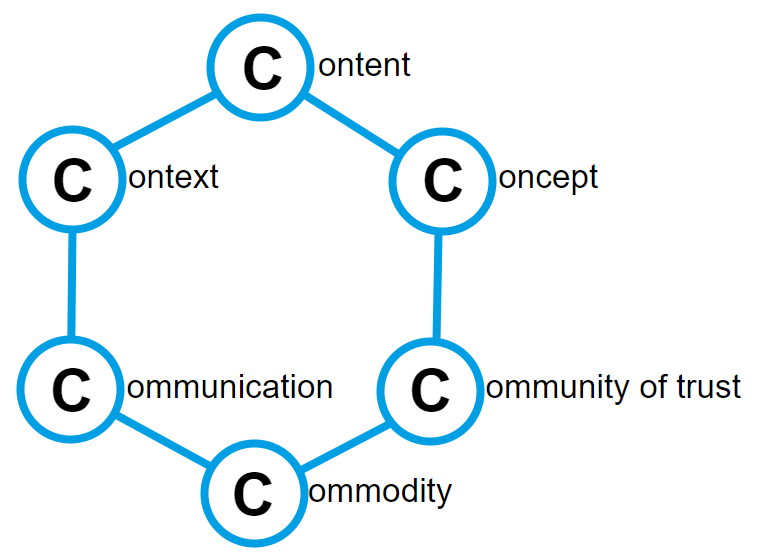
\includegraphics[width=3.64in,height=2.67in]{./media/image32.png}
		\caption{Outline of the Concern-Basic concern hexagon}
		\label{fig:Outline_of_the_ConcernBasic_concern_hexagon}
	\end{Center}
\end{figure}


%%%%%%%%%%%%%%%%%%%% Figure/Image No: 23 Ends here %%%%%%%%%%%%%%%%%%%%

\paragraph{Concern Hexagon\\}
%\addcontentsline{toc}{paragraph}{Concern Hexagon}
To illustrate the main modeling \uline{c}oncerns of Digital Resources in a way easy to memorize, the mnemonic hexagonal arrangement of \uline{c}arbon atoms can be used (C-Hexagon), as shown in Figure \ref{fig:Outline_of_the_ConcernBasic_concern_hexagon}. As a Resource’s content is its most essential aspect, Content is located at the top of the hexagon. This content is interpretable by references to a shared, formally defined Concept, whereas links to a particular \textit{C}ontext\textit{ }(in terms of time, place, or real-world entities) make the content potentially relevant for certain Data Consumers. So the upper part of the C-Hexagon deals with the "what" aspects, independently of Data Exchange, Data Sharing or Data Utilization. The lower part relates to the "how" aspects; i.e. how the content is exchanged (\textit{C}ommunication) and under which conditions (\textit{C}ommodity). The \textit{C}ommunity of Trust concern refers to the distinctive feature of the International Data Spaces being an ecosystem of certified participants and components that exchange and share Digital Resources in accordance with usage policies ensuring data sovereignty.

The level of detail differs across the individual concerns. The selection of their constituting aspects may change in light of new requirements and insights. Modeling concerns may inform, but do not necessarily correspond to any physical organization of the model (e.g., modules or directories). Some of the models listed below directly map to the above mentioned concerns, while others take a more detailed perspective on particular aspects.

\paragraph{Content\\}
%\addcontentsline{toc}{paragraph}{Content}


The \textit{Content }concern deals with the description of a Resource’s inherent substance, i.e. its $``$content$"$  available in any machine-interpretable, binary format. It addresses questions like: 
 \begin{itemize}
	\item What type of content does a Resource provide (e.g. text or an image)? 
 	\item What does the content look like (i.e. what is its structure, format etc.)? 
 	\item Is a content sample provided? 
 	\item What is the size and creation date of a particular file?
\end{itemize} 

At the abstract \textit{Resource} level, content is described independently of its physical manifestation. It is made concrete by augmenting structural information, i.e. details of how content is serialized into one of the supported \textit{Representations. }At a certain point in time, a Representation materializes in one or several \textit{Instances} (e.g. values or files). \\

\begin{figure}[H]
	\begin{Center}
		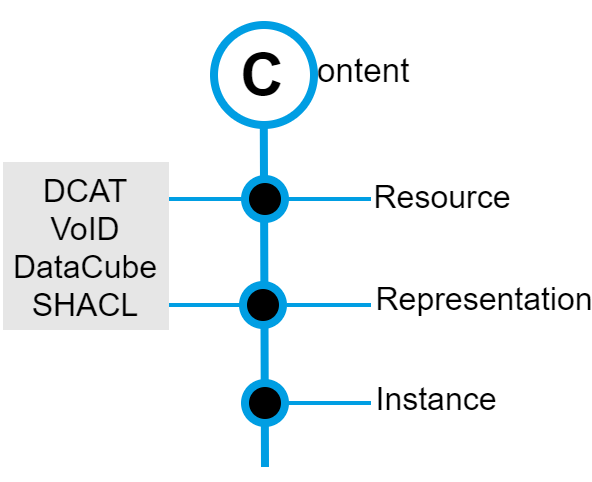
\includegraphics[width=2.0in,height=2.61in]{./media/image33.png}
		\caption{Outline Content Concern}
		\label{fig:outline_content_concern}
	\end{Center}
\end{figure}


\subparagraph*{Resource }
%\addcontentsline{toc}{subparagraph}{Resource}
Digital content at the Resource level of description abstracts away from a particular physical manifestation and deals with aspects that are shared equally by any of the content’s embodiments. 

Example: A \textit{report (i.e. Text, see below) containing figures regarding the utilization of European highways since 2000}.



\textbf{RESOURCE TYPE} There are various types of Digital Resources\footnote{ https://tools.ietf.org/html/rfc2046 },\footnote{\ \  http://dublincore.org/documents/dcmi-terms/$\#$ section-7 }. Resources may differ with regard to the intended purpose, the level of structuring, or the (sensory) requirements for its consumption and interpretation. Distinguished sets of properties are expected to evolve per Resource type, depending on their (future) use and relevance. 

Regarding the IDS-RAM, \textit{Data }is defined in alignment with ISO/IEC 2382:2015\footnote{ https://www.iso.org/standard/63598.html } (Information technology – Vocabulary)  as a statement of facts provided in a formalized, structured format intended primarily for machine processing (i.e. atomic values or arrangements of data fields, optionally defined by a schema). \textit{Text }represents a meaningful sequence of characters written in human language, which is intended for being read and interpreted by humans (or other intelligent agents) regardless of its Representation (e.g. document or screenshot image). \textit{Audio }refers to media content primarily intended for aural perception; consumption of such content normally requires an audio output device (i.e. a loudspeaker). \textit{Image }is static (i.e. time invariant) media content intended for visual perception, normally requiring a display device (i.e. a screen). \textit{Video }is dynamic (i.e. time variant) media content intended for visual and aural perception, combining the rendering requirements of Image and Audio as well as further requirements on processing (decoding etc.). \textit{Software} is a collection of machine-interpretable instructions, such as executable software (binary), program code (source), or fragments thereof; after optional preprocessing (compilation, installation etc.) its intended purpose is a subsequent execution exposing functionality. \textit{Opaque} is another, unspecified type of custom, binary content. The \textit{Container} is a collection of multiple (implicit) content elements that are distributed as a single unit (archive). 



%%%%%%%%%%%%%%%%%%%% Figure/Image No: 24 starts here %%%%%%%%%%%%%%%%%%%%

\begin{figure}[H]
	\begin{Center}
		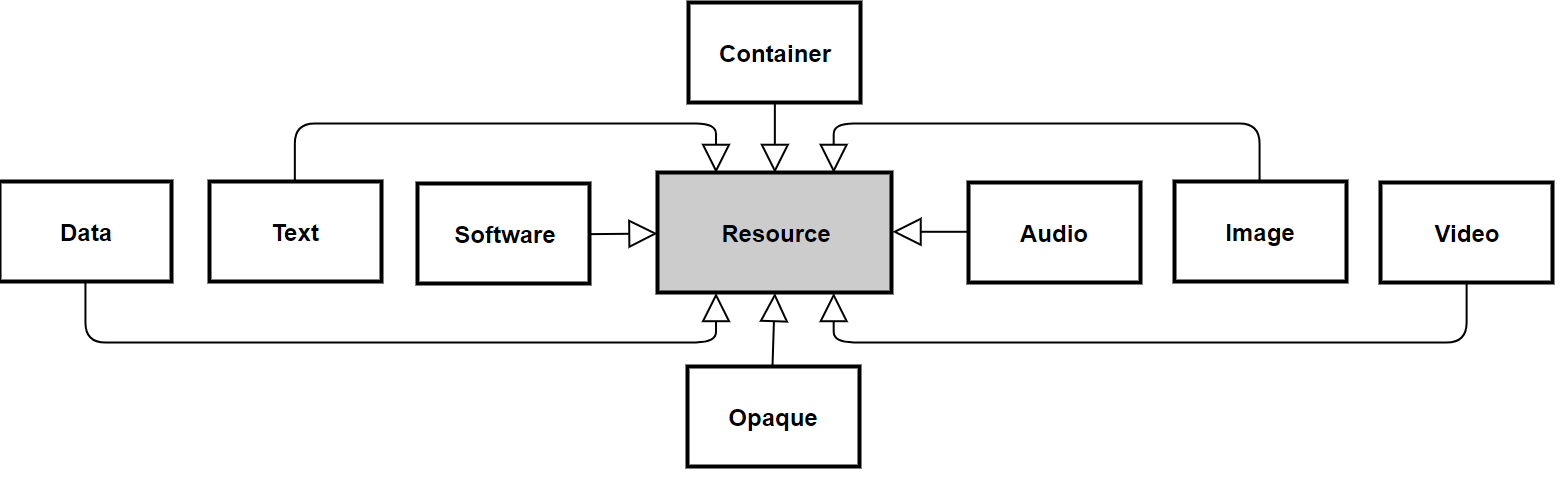
\includegraphics[width=6.53in,height=2.02in]{./media/image34.png}
		\caption{Taxonomy of the Resource concept}
		\label{fig:Taxonomy_of_the_Resource_concept}
	\end{Center}
\end{figure}


%%%%%%%%%%%%%%%%%%%% Figure/Image No: 24 Ends here %%%%%%%%%%%%%%%%%%%%



\textbf{HIERARCHY} Individual, physically or logically $``$included$"$  parts of the Container (e.g. an archive file), as well as any other structured Resource (e.g. software re-using 3\textsuperscript{rd} party libraries), may explicitly be referred to by the \textit{content-part} relation\footnote{http://dublincore.org/documents/dcmi-terms/$\#$ terms-hasPart }, allowing the modeling of part-whole hierarchies.

\textbf{CONTEXT} Temporal, spatial and real-world entities linked to the Resource content are covered by the Context concern (see section 3.4.3.6).

\textbf{CONCEPT} Semantic annotation of the Resource content is covered by the Concept concern (see section 3.4.6).



%%%%%%%%%%%%%%%%%%%% Figure/Image No: 25 starts here %%%%%%%%%%%%%%%%%%%%

\begin{figure}[H]
	\begin{Center}
		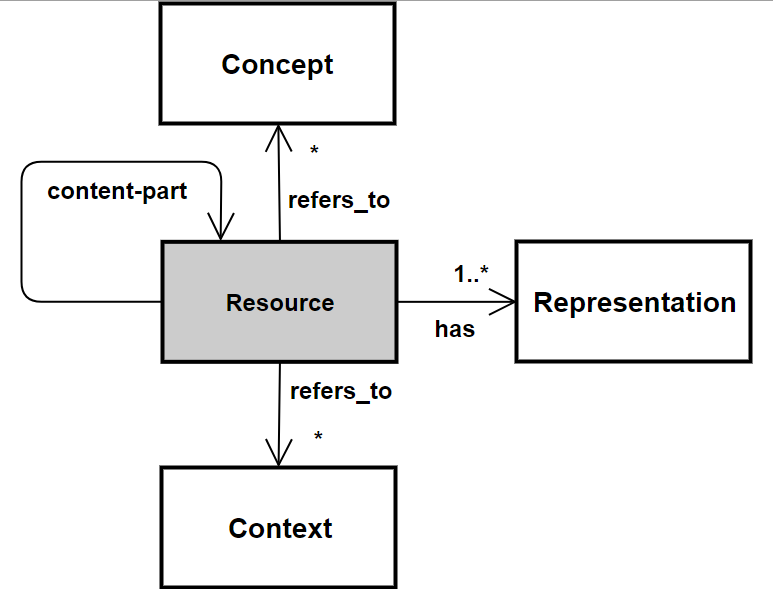
\includegraphics[width=3.44in,height=2.74in]{./media/image35.png}
		\caption{Resource concept (outline)}
		\label{fig:Resource_concept_outline}
	\end{Center}
\end{figure}


%%%%%%%%%%%%%%%%%%%% Figure/Image No: 25 Ends here %%%%%%%%%%%%%%%%%%%%


\subparagraph*{Representation}
%\addcontentsline{toc}{subparagraph}{Representation}
Abstract Resource content can be made $``$concrete$"$  by adding serialization details, i.e. by specifying alternative, physical Representations of the content. For example, Image content might be exposed via raster (JPEG, PNG, GIF) or vector graphics Representations (SVG). Developers of a „software for image anonymization$"$  might provide alternative software Representations (Windows EXE, Debian DEB, or Java JAR) supporting different software environments and operating systems. 

Example: \textit{The above mentioned report made available in a PDF or MS Word format}. 

\textbf{TYPE} The general physical arrangement of the content is indicated by the Internet Media Type (MIME-Type) and, if appropriate, more specifically by its specific data type.

\textbf{SCHEMA} Schema documents provide a formal structure definition of a Data Resource type. Profiles may add additional, selective constraints that apply to a subset of the considered data (e.g. geospatial data)\footnote{As an example, consider DCAT-AP, the DCAT Application Profile for data portals in Europe: https://joinup.ec.europa.eu/solution/dcat-application-profile-data-portals-europe }.

\textbf{PACKAGING} Packaging refers to means for archiving, compressing, and encrypting a Representation in a transparent, generic way.



%%%%%%%%%%%%%%%%%%%% Figure/Image No: 26 starts here %%%%%%%%%%%%%%%%%%%%

\begin{figure}[H]
	\begin{Center}
		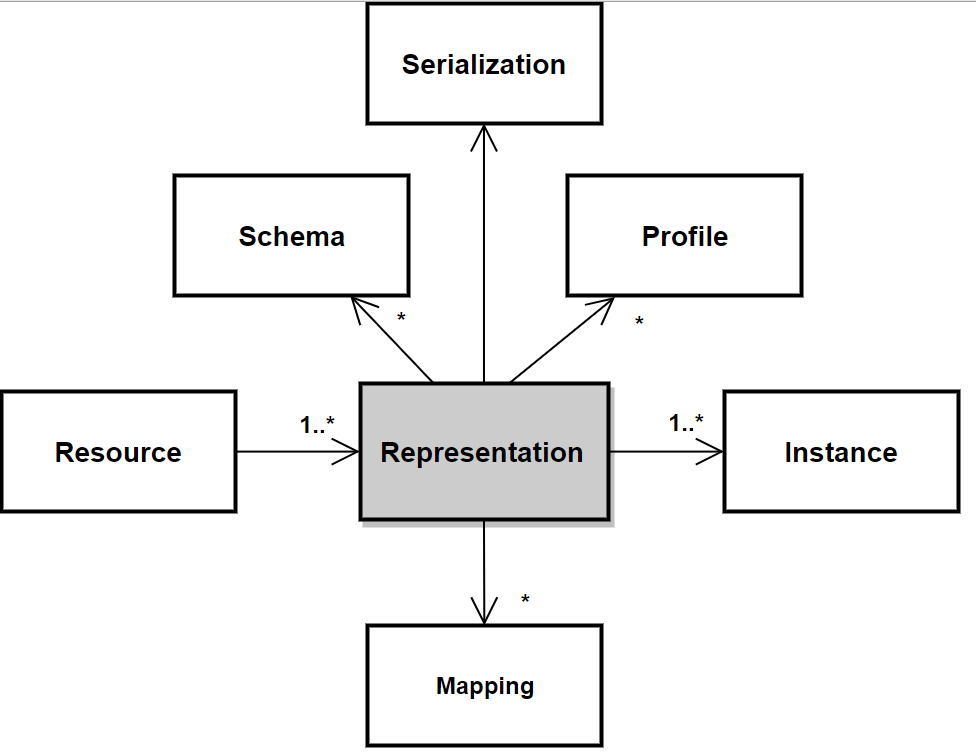
\includegraphics[width=4.03in,height=3.12in]{./media/image36.png}
		\caption{Representation concept (outline)}
		\label{fig:Representation_concept_outline}
	\end{Center}
\end{figure}


%%%%%%%%%%%%%%%%%%%% Figure/Image No: 26 Ends here %%%%%%%%%%%%%%%%%%%%


\subparagraph*{Instance}
%\addcontentsline{toc}{subparagraph}{Instance}
At a certain point in time, a Representation materializes into instances, which are either transient values or persisted files (Artifacts). Going beyond the prototypical level of Representation, an Instance captures properties that are unique to this materialization of the Resource’s content or particular elements thereof. 



Example: \textit{Version 3.1 of the above mentioned report; date of creation: 2018/01/17; file size: 1,73 MB (PDF) and 1,81 MB (MS Word), respectively}.



\textbf{IDENTITY} A rendered artifact may be provided with (partial) identity features, such as a file name or hash sum. It becomes identifiable and distinguishable from other artifacts, and is suited for file-oriented provision. (Representations, in contrast, are suited for interactive, service-oriented provision, due their nature of being prototypical „blueprints$``$.) 

\textbf{SIZE }The Size (specified e.g. in bytes) is another inherent characteristic of an artifact. 



\paragraph{Context\\}
%\addcontentsline{toc}{paragraph}{Context}
The \textit{Context} concern deals with temporal and spatial aspects as well as with real-world entities a Resource’s content relates to (intrinsic context). It addresses questions like: 
 \begin{itemize}
	\item What time period does the content cover? 
 	\item When and where was it gathered? 
 	\item Which sub-entity of a larger entity does a certain dataset relate to?
\end{itemize} 
Accurate context modeling helps a client in searching for and assessing the relevance of a Resource with respect to her informational needs, for example, by looking at most recent data (\textit{Time}) available for water pipelines (\textit{Entity}) within a particular area of interest (\textit{Space}) 


\begin{figure}[H]
	\begin{Center}
		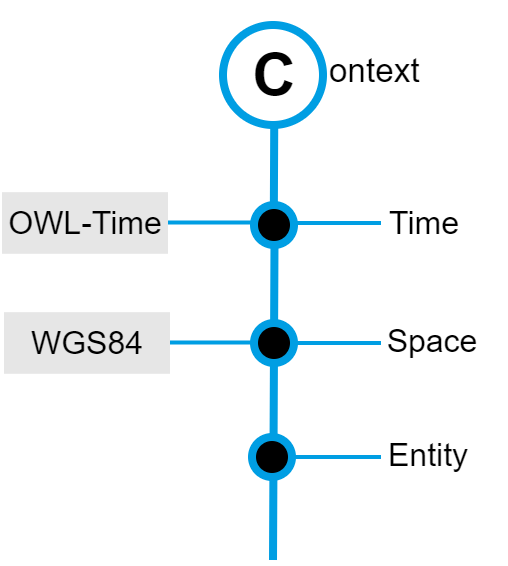
\includegraphics[width=1.33in,height=2.68in]{./media/image37.png}
		\caption{Outline Context Concern}
		\label{fig:outline_context_concern}
	\end{Center}
\end{figure} 


\subparagraph*{Time and space}
%\addcontentsline{toc}{subparagraph}{Time and space}
Time and space are quantifiable context dimensions usually expressed by coordinates with regard to a shared reference system, such as Coordinated Universal Time (UTC\footnote{https://www.itu.int/dms\_pubrec/itu-r/rec/tf/R-REC-TF.460-6-200202-I!!PDF-E.pdf }) or World Geodetic System 1984 (WGS 84\footnote{http://earth-info.nga.mil/GandG/publications/tr8350.2/wgs84fin.pdf }), allowing for unambiguous interpretation. One-dimensional temporal context is limited to either a single point in time (instant) or an interval with a non-empty duration. Thanks to the linear nature of time, open-end intervals may express a continuous period with only an endpoint defined\footnote{https://www.loc.gov/standards/datetime/edtf.html }. In contrast to temporal context, spatial context is capable of expressing two-dimensional and three-dimensional shapes as bounding boxes defined by a set of coordinates. 

Example: \textit{Time period covered by the report, starting at 01/01/2000 UTC (end time is undefined here, as the report is continuously updated)}. 


\subparagraph*{Real-world entities}
%\addcontentsline{toc}{subparagraph}{Real-world entities}
This type of \textit{qualitative} context refers to identifiable temporal and spatial entities, i.e. which are (implicitly) defined by spatio-temporal coordinates. These are conventionalized \textit{named entities}, such as time periods\footnote{https://en.wikipedia.org/wiki/List\_of\_time\_periods } ($``$Renaissance$"$ ), country codes (according to ISO 3166\footnote{https://www.iso.org/iso-3166-country-codes.html }), national\footnote{https://de.wikipedia.org/wiki/Liste\_der\_Bundesautobahnen\_in\_Deutschland } and international road names (ECE/TRANS/SC.1/2016/3/Rev.1\footnote{https://www.unece.org/trans/main/sc1/sc1doc\_2016.html }) etc. Being based upon an established reference system, standard, or convention, such entities are considered universally valid. In addition, within restricted domains (e.g. a building), \textit{custom context entities} may be defined (e.g. individually numbered rooms), serving the purposes of contextualizing data (e.g. for sensor observations). The usability of custom context entities is limited by the characteristics of the defining model, i.e. being a machine-interpretable, widely accepted one \textbf{(}ISO 16739\footnote{https://www.iso.org/standard/70303.html }), and the context entities themselves. These should have a (semantic) type or \textit{concept} information attached in order to support general, categorical queries for data (e.g. temperature sensed in all $``$laboratories$"$ ). This type of annotation is, among others, supplied by the \textit{Concept }concern. 

Example: \textit{$``$A 555$"$ , Germany’s first highway ever built, connecting the cities of Bonn and Cologne, which is mentioned in the report}. 

\paragraph{Concept\\}
%\addcontentsline{toc}{paragraph}{Concept}
 The \textit{Concept }concern deals with the modeling of the $``$meaning$"$ , annotation, and interpretation of entities introduced by the orthogonal Resource concerns (Content, Context, Communication etc.). It addresses questions like:  \begin{itemize}
	\item What type of observation does the data refer to $``$temperature$"$  ? 
 	\item What kind of object does a context entity represent (factory, building)? 
 	\item What is the meaning of a certain date parameter (beginning or end of a range)?
\end{itemize} 
 \textit{Keywords }express the $``$meaning$"$  of an entity via informal natural language tags. As keywords can be chosen freely by a Data Provider, they are prone to inconsistencies and errors. Using controlled vocabularies, it is possible to add curated, (formally) defined and reusable \textit{Terms}, which can be shared across different scenarios and domains. In addition, conceptual schemas and ontologies define \textit{Types} of entities, if these are to be individually modeled as custom instances.  

\begin{figure}[H] 			
	\begin{Center}
		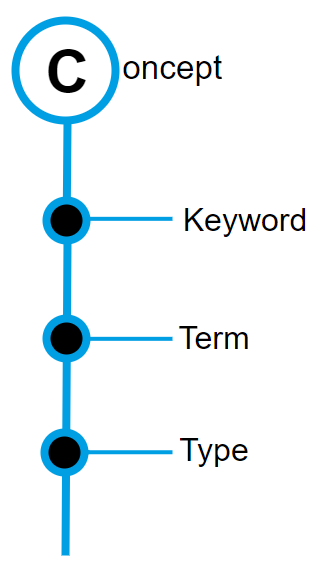
\includegraphics[width=1.46in,height=2.77in]{./media/image38.png}
		\caption{Outline Concept Concern}
		\label{fig:outline_concept_concern}
	\end{Center}
\end{figure}

\textbf{KEYWORD} Keywords are natural language annotations (tags) arbitrarily chosen by the Data Provider to accurately characterize the Resource from their perspective. As such, they are likely to be subjective and more domain specific than general terms provided by controlled vocabularies. Consistency and alignment of custom tag sets can be supported by means of documentation (guidance), editing tools (tag suggestions), or quality gates during the publication process, for example. 

Examples: \textit{$``$statistics$"$ , $``$highway$"$ , $``$usage$"$ , $``$traffic$"$ , $``$Europe$"$ .}

\textbf{TERM} In contrast to (arbitrarily chosen) keywords, terms are normally retrieved from an authoritative, curated source of definition (controlled vocabulary) or defined as instances of a conceptual type system. Identified by a normative literal (code) or a unique identifier (URI), each term represents a reusable concept ($``$singleton$"$ ) that can be shared across different usage scenarios and domains without variations. 

Example: \textit{http://example.org/traffic\_statistics}. 

\textbf{TYPE} Terms are not capable of expressing individual characteristics of annotated entities. For this purpose, conceptual schemas and ontologies define \textit{types} of entities (e.g. classes, concepts) along with properties and relations their instances may adopt. Unlike terms, instances of a type convey the custom, particular semantics of the modeled entity. Conceptual types may be extended (specialized) to meet the requirements of other domains. 

Example: \textit{http://example.org/TabularTrafficReport.}\par

\paragraph{Communication\\}
%\addcontentsline{toc}{paragraph}{Communication}


The \textit{Communication }concern deals with means to communicate a Resource’s content in one of the Representations available. It addresses questions like:  \begin{itemize}
	\item Is there any input required on client to retrieve the content?  	
	\item What communication protocols are supported? 
 	\item What does a valid request look like? 
 	\item What is the address of the endpoint handling the request?
\end{itemize} 
 \textit{Operations} are the building blocks of interactive interfaces for sharing and processing a Resource’s content. They model an abstract functionality along with involved parameters and underlying interaction patterns. Through bindings to a communication protocol, operations become $``$concrete$"$  and can be invoked at networked \textit{Endpoints}. A Connector’s interactions at these Endpoints can be complemented by \textit{Message} metadata.


\begin{figure}[H]
	\begin{Center}
		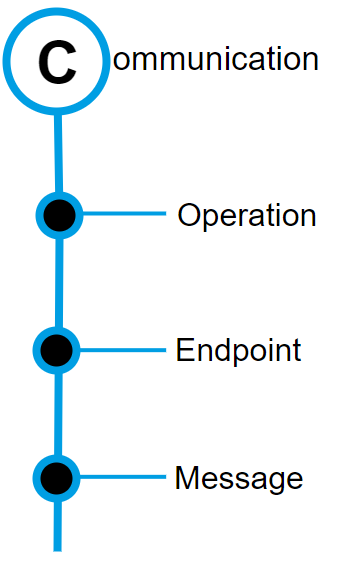
\includegraphics[width=1.36in,height=2.5in]{./media/image39.png}
		\caption{Outline Communication Concern}
		\label{fig:outline_communication_concern}
	\end{Center}
\end{figure}



\subparagraph*{Operation}
%\addcontentsline{toc}{subparagraph}{Operation}
An operation models an atomic unit of functionality in the exchange, processing, visualization, or persistence of digital content. Operations related to each other may be grouped into service interfaces (i.e., sets of a coherent functionality defining an abstract $``$interaction contract$"$ ). 

Example: \textit{Read operation providing access to a parameterized report (may expect a start year parameter, an end year parameter, or both)}. 

\textbf{PARAMETER} Parameters are named slots of an operation’s interface. They define the least level of content granularity an operation may (optional) or must (mandatory) expect as an input or output. Each parameter mediates a particular kind of digital content. This is defined by reusing the triadic content model from Section 3.4.3.5. Thereby abstract aspects (i.e. the meaning) and concrete aspects (i.e. the shape) of the parameter are covered. Optionally, the default value or lists of selectable, enumerated values can be defined as instances of that content model. Additional parameter types (e.g., an ID or the start or end of a period) provide information for operation clients about the purpose and intended usage of the parameter and may e.g. support a query generation process. 

Example: \textit{Parameter indicating a year within the period between 2000 and 2018 (further categorized as the start of a date range)}. 

\textbf{OPERATION TYPE} The type conveys the semantics (i.e., the functional capabilities) of an operation. Building upon conventions established within technology related communities (e.g., REST-architecture paradigm\footnote{https://www.ics.uci.edu/$ \sim $ fielding/pubs/dissertation/rest\_arch\_style.htm }), a taxonomy of operation types (interaction primitives) has been defined for the purpose of Resource exchange, as depicted in \textbf{Fehler! Verweisquelle konnte nicht gefunden werden.}. 



%%%%%%%%%%%%%%%%%%%% Figure/Image No: 27 starts here %%%%%%%%%%%%%%%%%%%%

\begin{figure}[H]
	\begin{Center}
		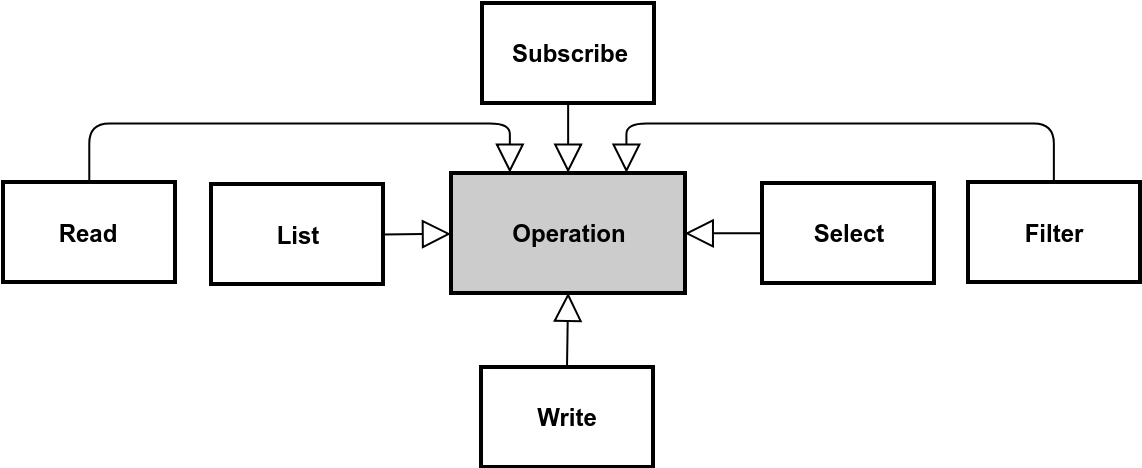
\includegraphics[width=4.15in,height=1.7in]{./media/image40.png}
		\caption{Taxonomy of Operation types for Resource exchange}
		\label{fig:Taxonomy_of_Operation_types_for_Resource_exchange}
	\end{Center}
\end{figure}


%%%%%%%%%%%%%%%%%%%% Figure/Image No: 27 Ends here %%%%%%%%%%%%%%%%%%%%



A client may\textit{ read} the digital content of a single, identified Resource, or \textit{list} a collection of resources. By providing an appropriate expression (e.g., an XPath selector\footnote{https://www.w3.org/TR/xpath-31/ }), the client may \textit{select } a subset of matching resources or \textit{filter } for relevant content fragments (e.g., via an LDAP filter\footnote{https://tools.ietf.org/search/rfc4511$\#$ section-4.5.1 }). The client may \textit{subscribe} for proactive content pushed by the Data Provider, given the permission to \textit{write} (or deliver) the content. Some operation types may impose constraints on type and number of parameters required, as demonstrated by the $``$select$"$  and $``$filter$"$  parameters above.

\textbf{PATTERN }The order of supplying the operation parameters is governed by the operation’s interaction pattern, comparable to web service Message Exchange Patterns\footnote{https://www.w3.org/TR/wsdl20-adjuncts/$\#$ meps } (MEP). For example, the $``$out-only$"$  pattern indicates an unreliable (possibly asynchronous) server-side notification, extended in $``$robust-out-only$"$  pattern by a mandatory confirmation. Such a $``$reliable notification$"$  may be implemented in a variety of ways, depending on the communication protocol and the programming paradigm used.

Example: \textit{In-out interaction pattern, since the result depends on (optional) input parameters}.


%%%%%%%%%%%%%%%%%%%% Figure/Image No: 28 starts here %%%%%%%%%%%%%%%%%%%%

\begin{figure}[H]
	\begin{Center}
		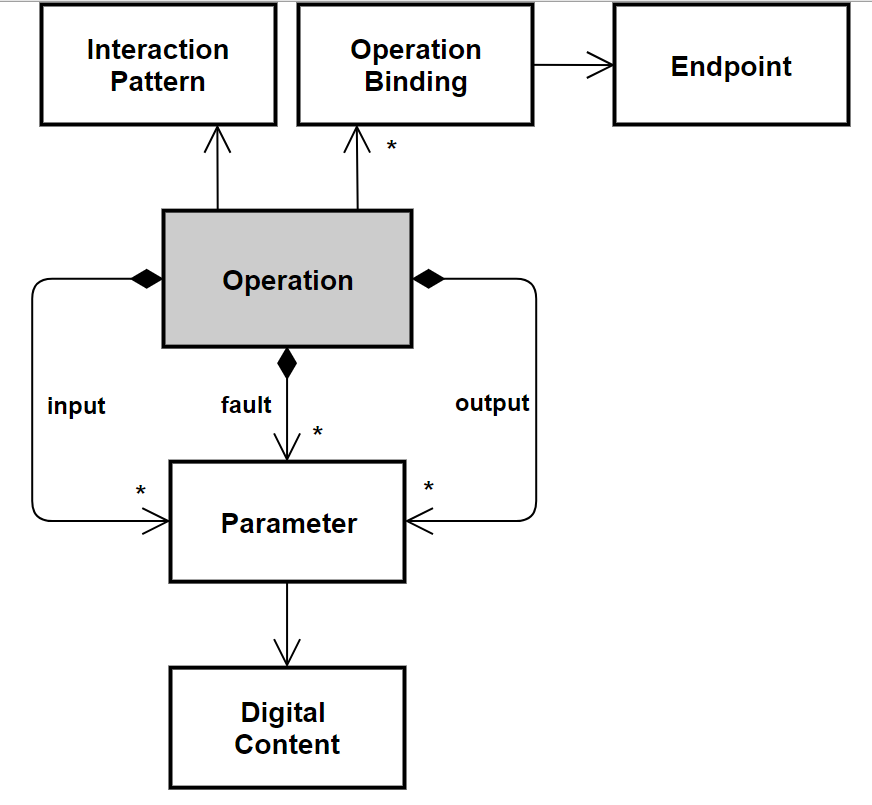
\includegraphics[width=3.08in,height=2.84in]{./media/image41.png}
		\caption{Operation concept (outline)}
		\label{fig:Operation_concept_outline}
	\end{Center}
\end{figure}


%%%%%%%%%%%%%%%%%%%% Figure/Image No: 28 Ends here %%%%%%%%%%%%%%%%%%%%


\subparagraph*{Endpoint}
%\addcontentsline{toc}{subparagraph}{Endpoint}
An Endpoint is a concrete point of content exchange (Resource Endpoint) and service interaction (Service Endpoint) that is uniquely identifiable via a specific communication protocol.

Example: \textit{https://stathub.org/report?start=$ \{ $ year1$ \} $ $\&$ end=$ \{ $ year2$ \} $ }.

\textbf{BINDING }An individual operation or an entire interface can be invoked at an Endpoint by bindings to communication protocols (such as HTTP/2\footnote{https://tools.ietf.org/html/rfc7540 }) by means of established, machine-readable interface description languages (e.g., Open API\footnote{https://www.openapis.org/ }).

\textbf{HOST }The address scheme type (e.g., HTTPS URL, MQTT topic) and communication protocol are defined by the implementing host, which is a server node installed within a Connector. Within the address space of the host, each Endpoint is registered at a particular path, topic, or queue. 

\subparagraph*{Message}
%\addcontentsline{toc}{subparagraph}{Message}
In contrast to the general communication capabilities described above, the Message concept describes the content payload being exchanged at runtime between Connectors. Message metadata provides traceable evidence of the communication (e.g. addresses, transaction ID) and allows interpretation of the context (i.e. type of content, usage contract) within which an Instance of a Resource’s digital content is mediated. Depending on the implementation, this metadata may be supplied as a standalone part of an initial session negotiation or as an integral part of the content transfer (e.g., as header part of a compound multi-part message\footnote{https://tools.ietf.org/html/rfc7578 }). Thus, the Message metadata may either complement interactions of legacy application protocols or may be used independently as a foundation for modeling the exchange of the Resource in a generic, technology-agnostic manner. In the latter case, each state of the interaction is mapped onto an instance of an appropriate Message type (ArtifactRequestMessage). 

Example:\  \textit{Message of the $``$ArtifactRequestMessage$"$  type requesting provision of the artifact named $``$Report\_2000-2010.pdf$"$ }. 

\textbf{MESSAGE TYPE }\textbf{Fehler! Verweisquelle konnte nicht gefunden werden.} illustrates an excerpt of the Message taxonomy. Request-response interactions between the Connectors of interacting participants are reflected by the dedicated subclasses of the RequestMessage and the RequestResponse type. Event-like notifications are reflected by the NotificationMessage subclasses.



%%%%%%%%%%%%%%%%%%%% Figure/Image No: 29 starts here %%%%%%%%%%%%%%%%%%%%

\begin{figure}[H]
	\begin{Center}
		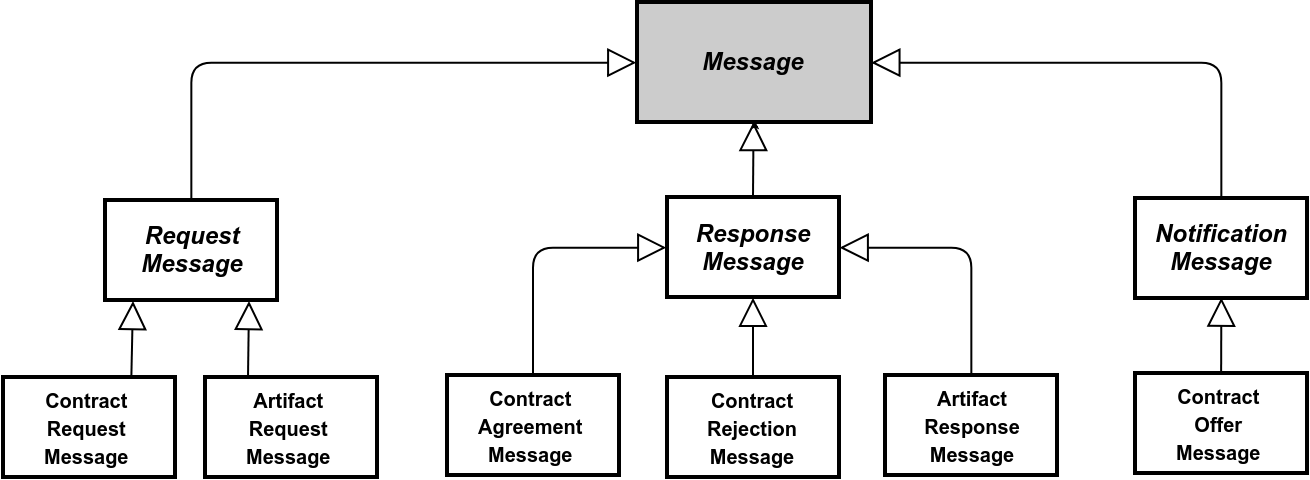
\includegraphics[width=4.5in,height=1.65in]{./media/image42.png}
		\caption{Message taxonomy (excerpt)}
		\label{fig:Message_taxonomy_excerpt}
	\end{Center}
\end{figure}


%%%%%%%%%%%%%%%%%%%% Figure/Image No: 29 Ends here %%%%%%%%%%%%%%%%%%%%


\textbf{ADDRESSING }The Message identifies the participants involved in the interaction (e.g. a Data Provider and a Data Consumer), as well as their Connectors, allowing for routing, provenance tracking, and clearing, among other things.

\textbf{SECURITY} The Security aspect covers, among other things, the authorization features of the client (e.g., JSON Web token\footnote{https://jwt.io/ }) and references to the contract underlying the interaction. 

\paragraph{Commodity\\}
%\addcontentsline{toc}{paragraph}{Commodity}


The \textit{Commodity} concern helps assess the value and utility of a Resource as an obtainable asset with regard to a client’s needs. It addresses questions like:
 \begin{itemize}
	\item Does the Resource origin from a reliable source? 
 	\item What level of quality does the Resource have? 
 	\item What are the restrictions regarding the use of the Resource? 
 	\item How much does it cost to use the Resource?
\end{itemize} 
 \textit{Provenance} explicates the context of the Resource’s creation and its history of modification. The \textit{Quality} of a Resource’s content and provisioning services may be assessed by means of tests, quality of service (QoS) parameters, and ratings from previous users in the community. The \textit{Policy }determines the conditions for using the Resource, including \textit{Pricing}, in a formal way supporting contract negotiation and (automated) contract enforcement. 

\begin{figure}[H]
	\begin{Center}
		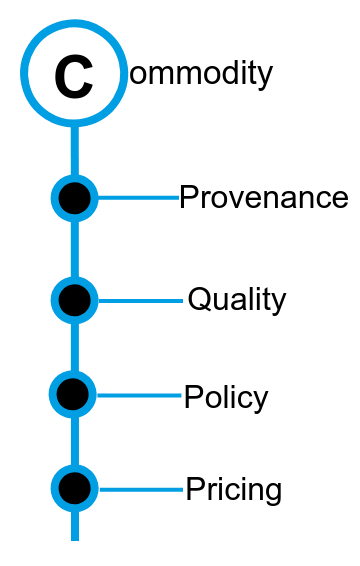
\includegraphics[width=1.34in,height=2.33in]{./media/image43.png}
		\caption{Outline Commodity Concern}
		\label{fig:outline_commodity_concern}
	\end{Center}
\end{figure}


\subparagraph*{Provenance}
%\addcontentsline{toc}{subparagraph}{Provenance}
Provenance is concerned with the origin of the digital content,, the history of modifications it has undergone, and the agents responsible for these activities. The main goal of provenance tracking is to ensure reliability of the content, so that modifications are made explicit and comprehensible and may be analyzed for defects. Furthermore, provenance information should refer to the socio-economical context of the content’s creation (the project the content was created in, who the project was funded by etc.) in order to assess the underlying motivation, potential limitations, or bias. 

Example: \textit{Report v3.1, derived from v3.0, including additional tables and diagrams added by John Doe on 2018/01/17}.



\textbf{AGENT} An Agent is any organization, person, or software that has conducted or influenced an Activity. Agents are not necessarily registered participants of the International Data Spaces. Precautions should be taken to ensure a sufficient description of such external Agents is supplied.

\textbf{ACTIVITY} An Activity is a notable, temporarily limited operation applied by an Agent upon the content in question (such as content creation, transformation, usage, or sharing). The vocabulary of Provenance Activities should be controlled (i.e. guidance should be provided to ensure homogeneous annotation and evaluation/querying).


\textbf{CONTENT} Compared to generic provenance models, such as the PROV Ontology\footnote{ https://www.w3.org/TR/prov-o/ }, the IDS provenance model focuses on uniquely identifiable digital content as a subject to Activities along the Provenance tracking. Depending on the type of Activity, this may link to abstract content (creation), concrete content (specification), or materialized content (modification). 



%%%%%%%%%%%%%%%%%%%% Figure/Image No: 30 starts here %%%%%%%%%%%%%%%%%%%%

\begin{figure}[H]
	\begin{Center}
		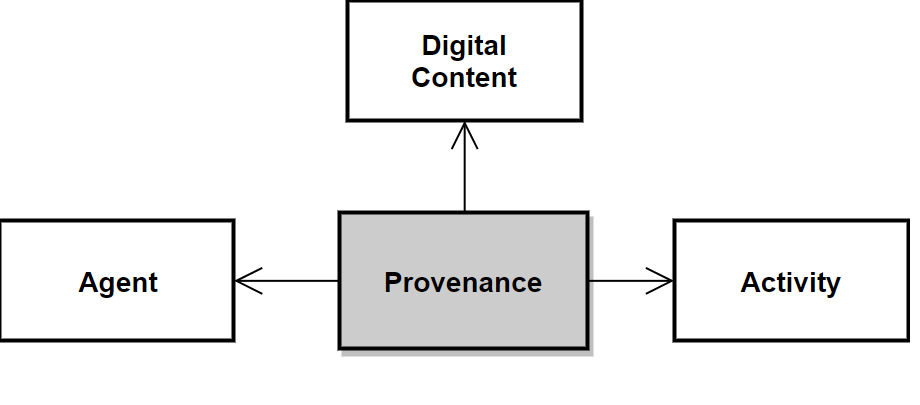
\includegraphics[width=3.74in,height=1.65in]{./media/image44.png}
		\caption{Provenance concept (outline)}
		\label{fig:Provenance_concept_outline}
	\end{Center}
\end{figure}


%%%%%%%%%%%%%%%%%%%% Figure/Image No: 30 Ends here %%%%%%%%%%%%%%%%%%%%


\subparagraph*{Quality}
%\addcontentsline{toc}{subparagraph}{Quality}
Quality is commonly interpreted as $``$fitness for use$"$  (J. M. Juran)\footnote{Juran, J.M., Juran on Planning for Quality. 1988, New York: The Free Press.  }, emphasizing the contextual nature of quality. Data Consumers can assess the fitness of a data offering for their needs based on quality statements supplied alongside with the Resource. These are, among other things, quality assessments according to a multidimensional model (e.g. ISO/IEC 25012 data quality model\footnote{https://iso25000.com/index.php/en/iso-25000-standards/iso-25012 }), a certificate of quality, or any form of community feedback.


\textbf{DIMENSION} A quality Dimension is a qualitative characteristic of a dataset relevant to the Data Consumer. It relates to whether data is complete, valid, accurate, up to date, (technically) available, and so on. User-oriented quality dimensions are measured by means of one or more quantifiable metrics. 

\textbf{METRIC} A quality Metric implements a particular approach to assess a data quality dimension by observing a concrete indicator, such as the spatial resolution (accuracy) or the up-time of the Resource’s server (availability). The value of a metric is often numeric (percentage) or boolean. 

\textbf{MEASUREMENT} Evaluation of a given dataset against a specific quality metric results in a measurement. Measurement results, as well as individual, subjective assessments may be annotated by means of metadata. 

\textbf{METADATA} Quality related metadata provides provenance information, information about the agent that performed the overall evaluation or an individual measurement (quality checker), information about the source it was originally derived from (accumulative metrics), and the time of evaluation.

\textbf{CERTIFICATE} A quality Certificate is a document that certifies the quality of a Resource according to a set of quality assessment rules, such as the ODI Quality Certificate\footnote{https://certificates.theodi.org/ }. 

\textbf{FEEDBACK }The Feedback comprises any kind of community feedback regarding experiences made with certain data (such as star ratings, issue reports, or recommendations). Feedback considerably affects the credibility of data.



%%%%%%%%%%%%%%%%%%%% Figure/Image No: 31 starts here %%%%%%%%%%%%%%%%%%%%

\begin{figure}[H]
	\begin{Center}
		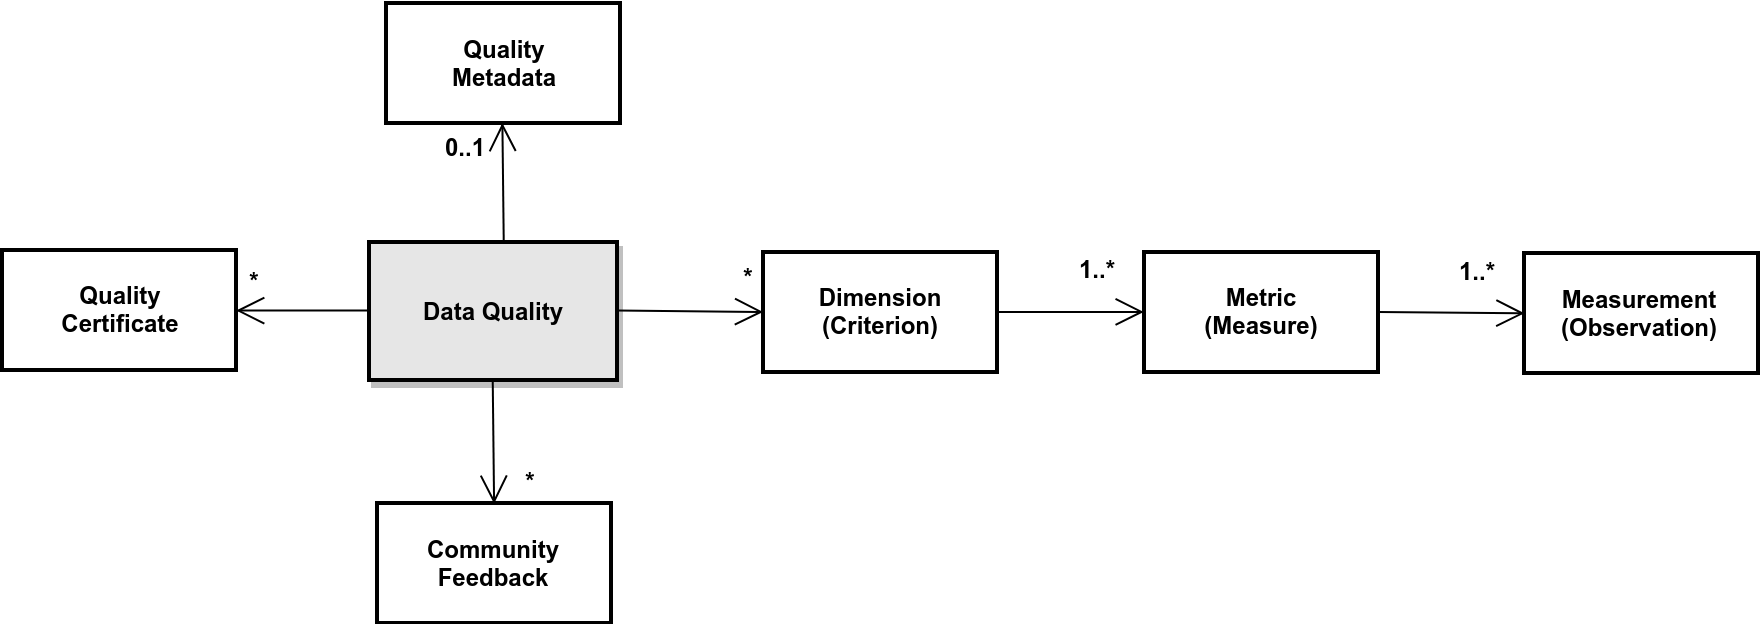
\includegraphics[width=6.53in,height=2.31in]{./media/image45.png}
		\caption{Outline of the: Data Quality concept (outline)}
		\label{fig:Outline_of_the_Data_Quality_concept_outline}
	\end{Center}
\end{figure}


%%%%%%%%%%%%%%%%%%%% Figure/Image No: 31 Ends here %%%%%%%%%%%%%%%%%%%%




\subparagraph*{Policy}
%\addcontentsline{toc}{subparagraph}{Policy}
A Policy defines rules for access to and usage of Resources. Published as part of a Resource’s metadata, it constitutes a contract offer to be further negotiated and agreed upon by the prospective Data Consumer. 

Example: \textit{Permission for unrestricted usage of report data given the obligation the assignee John Doe will cite the source of data (Creative Commons Attribution, CC by)}.

\textbf{RULE} A Rule defines Actions that an involved Party is obliged (Duty), permitted (Permission) or prohibited (Prohibition) to do with respect to an Asset.

\textbf{PARTY }The Parties involved in a data exchange transaction (i.e. the Data Owner/Provider and the Data Consumer, or their representative agents) are referred to by their respective roles, assigner and assignee. 

\textbf{ACTION} Alongside with operations on Assets (e.g. copy, print, convert), an Action may comprise general obligations (e.g. pay, attribute) or modify the interpretation of the policy (e.g. ensure exclusiveness)\footnote{https://www.w3.org/TR/odrl-vocab/$\#$ actionConcepts }. 

\textbf{ASSET }An Asset is the subject of a Rule, a Resource or a collection of Resources. Depending on the Policy’s specifications (e.g. do not redistribute), the Asset’s content needs to be identified in a persistent and unambiguous manner in order to be effectively enforceable, independently of the provisioning type (e.g. download URL) or storage context (Data Provider or Data Consumer) (for example, by an identifier composed of indicators such as artifact name and hash sum).

\textbf{CONSTRAINT} A formal Constraint may restrict the applicability of a Rule (e.g. by purpose of use), guide the selection of collection items (e.g. according to the file format) and permissible Parties (e.g. by role), or refine the interpretation of Actions (e.g. print at low resolution). The underlying Policy language has to define appropriate properties (e.g. purpose, file format, role, or resolution) along with conditions of their applicability and interpretation\footnote{https://www.w3.org/TR/odrl-vocab/$\#$ term-LeftOperand }. Reusing quality metrics (e.g. server uptime), as introduced above, allows specifying Policies on the required quality of service (QoS). 



%%%%%%%%%%%%%%%%%%%% Figure/Image No: 32 starts here %%%%%%%%%%%%%%%%%%%%

\begin{figure}[H]
	\begin{Center}
		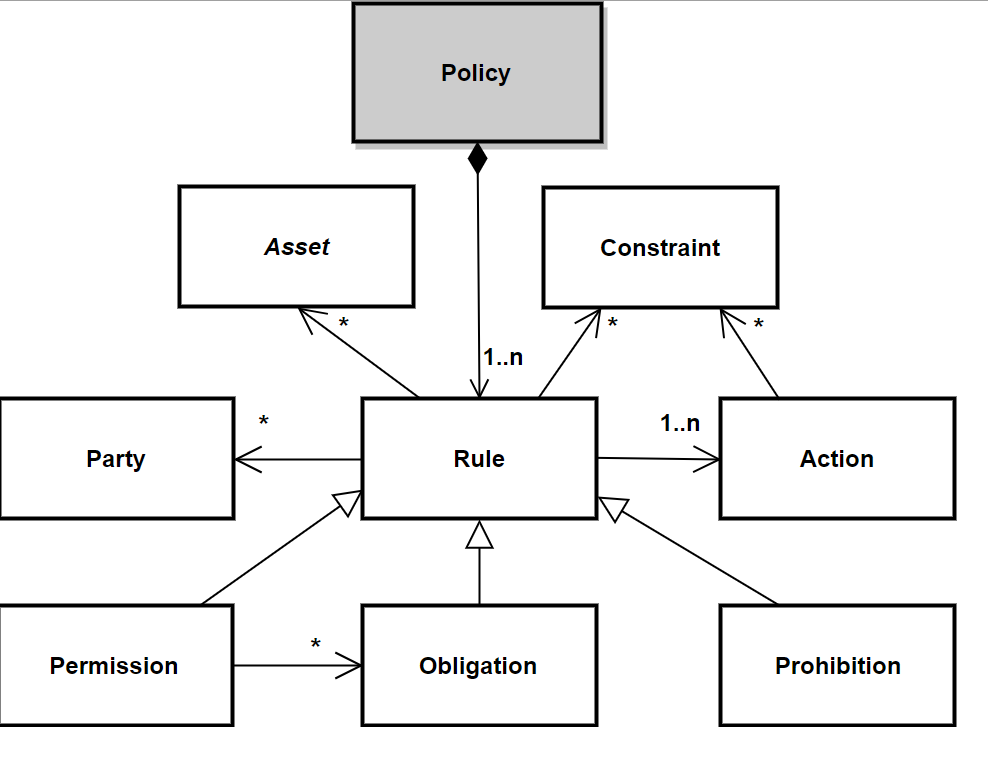
\includegraphics[width=4.14in,height=3.22in]{./media/image46.png}
		\caption{Policy concept (outline)}
		\label{fig:Policy_concept_outline}
	\end{Center}
\end{figure}


%%%%%%%%%%%%%%%%%%%% Figure/Image No: 32 Ends here %%%%%%%%%%%%%%%%%%%%



\subparagraph*{Pricing}
%\addcontentsline{toc}{subparagraph}{Pricing}
Pricing models applied to Resources exchanged in the International Data Spaces may vary. Applying a \textit{Free Use }model, the use of Resources is not charged (while other obligations may still apply, e.g. attribution). The \textit{Freemium} model exposes limited parts (or capabilities) of a Resource at no cost, while for additional parts particular subtypes of \textit{Chargeable Use} apply. The \textit{Quantity-based Pricing} model relies on particular quantitative metrics (e.g. volume, access count, download) to define a charged instance of usage (i.e. pay-per-use). The \textit{Feature-based Pricing} model depends on a selection of content features and quality parameters, such as map layers (basic, mobility, crime), image or audio resolution (low, high) etc. The least restrictive Pricing model, the \textit{Flatrate} model, allows unconstrained use of a Resource at a fixed price, but can potentially be limited by quantitative boundaries (such as bandwidth, number of parallel requests, or data transfer speed).

 Example: \textit{The European highway utilization report is provided free of charge}.


%%%%%%%%%%%%%%%%%%%% Figure/Image No: 33 starts here %%%%%%%%%%%%%%%%%%%%

\begin{figure}[H]
	\begin{Center}
		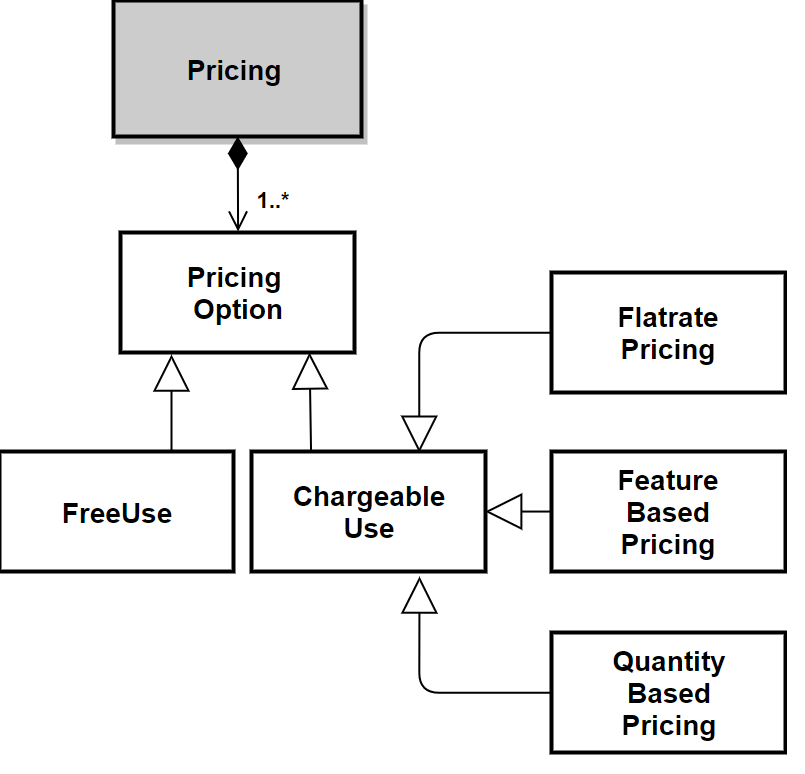
\includegraphics[width=2.7in,height=2.6in]{./media/image47.png}
		\caption{Pricing concept (outline)}
		\label{fig:Pricing_concept_outline}
	\end{Center}
\end{figure}


%%%%%%%%%%%%%%%%%%%% Figure/Image No: 33 Ends here %%%%%%%%%%%%%%%%%%%%



\paragraph{Community of trust\\}
%\addcontentsline{toc}{paragraph}{Community of trust}
The \textit{Community of trust} concern considers the fundamental requirement of the International Data Spaces for exchanging and sharing digital content between a Data Provider and a Data Consumer in a secure and trusted way, while preserving data sovereignty of the Data Owner. It addresses questions like: 
 \begin{itemize}
	\item What is known about the respective counterpart of the intended data exchange transaction? 
 	\item Is the respective system reliable with regard to technical guarantees? 
 	\item Is there a formal proof of the above, e.g. a valid certification? 
 	\item What are the restrictions regarding the use of the acquired content?
\end{itemize} 
 \textit{Participants }registered with the IDS provide or consume digital content by means of a dedicated software component: the \textit{Connector. }Participants and Connectors may undergo a formal \textit{Certification }process (depending on the role a Participant wants to assume in the IDS), stating their trustworthiness according to the criteria catalog and the extent of applied evaluation. Finally, the technical and legal terms of providing and consuming digital content are laid down in a formal \textit{Contract}.


\begin{figure}[H]
	\begin{Center}
		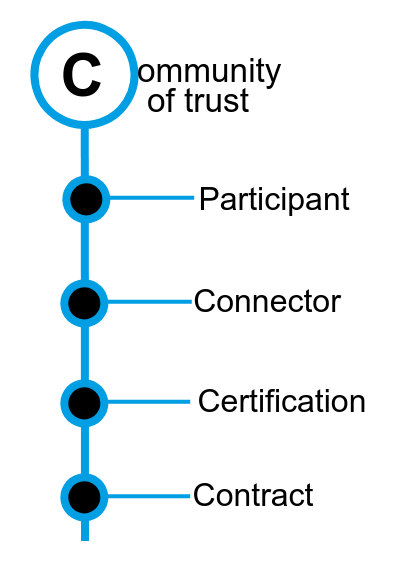
\includegraphics[width=1.36in,height=2.12in]{./media/image48.png}
		\caption{Outline Community of trust Concern}
		\label{fig:community_of_trust_concern}
	\end{Center}
\end{figure}


\subparagraph*{Participant}
%\addcontentsline{toc}{subparagraph}{Participant}
A Participant is a legal or natural person assuming a role (or more than one role) in the International Data Spaces. Participants must undergo a formal certification process.  

Example: \textit{AAStat, a public agency maintaining an infrastructure for monitoring, analysis, and prediction of highway statistics in Germany, has branches in Bonn and Berlin; since it provides open data that is available without any liability, it has refrained from undergoing an expensive certification process}.

\textbf{IDENTITY} Participants are registered at the International Data Spaces with a digital identity (X.509 certificate), alongside with other established, external identifiers (such asthe D-U-N-S Number\footnote{https://www.dnb.com/duns-number/ }). In accordance with linked-data principles, a Participant should always be unambiguously identifiable by a resolvable HTTPS URL, which links to a live metadata document describing the Participant.

\textbf{STRUCTURE} Organizations may link to individual employees, departments, or subsidiaries in order to allow for sharing authorizations, corporate policies etc. across the International Data Spaces. 

\textbf{SITE} Each Participant is associated with at least one site that serves the purpose of addressing geo-spatial queries (for reasons of proximity) or finding out about the local law in force. 

\textbf{BUSINESS} Participants may indicate the type of business and the domain in which they operate by making references to an established business classification (such as NAICS\footnote{https://www.census.gov/cgi-bin/sssd/naics/naicsrch?chart=2017 } or ISIC\footnote{https://unstats.un.org/unsd/publication/seriesm/seriesm\_4rev4e.pdf }). This information may support clients searching for digital content by business category. 

\textbf{CERTIFICATION} Depending on the role a Participant wants to assume in the IDS, the Participant may choose (or be required) to undergo an evaluation process resulting in a certification that states its compliance with a criteria catalog based on an evaluation method.



%%%%%%%%%%%%%%%%%%%% Figure/Image No: 34 starts here %%%%%%%%%%%%%%%%%%%%

\begin{figure}[H]
	\begin{Center}
		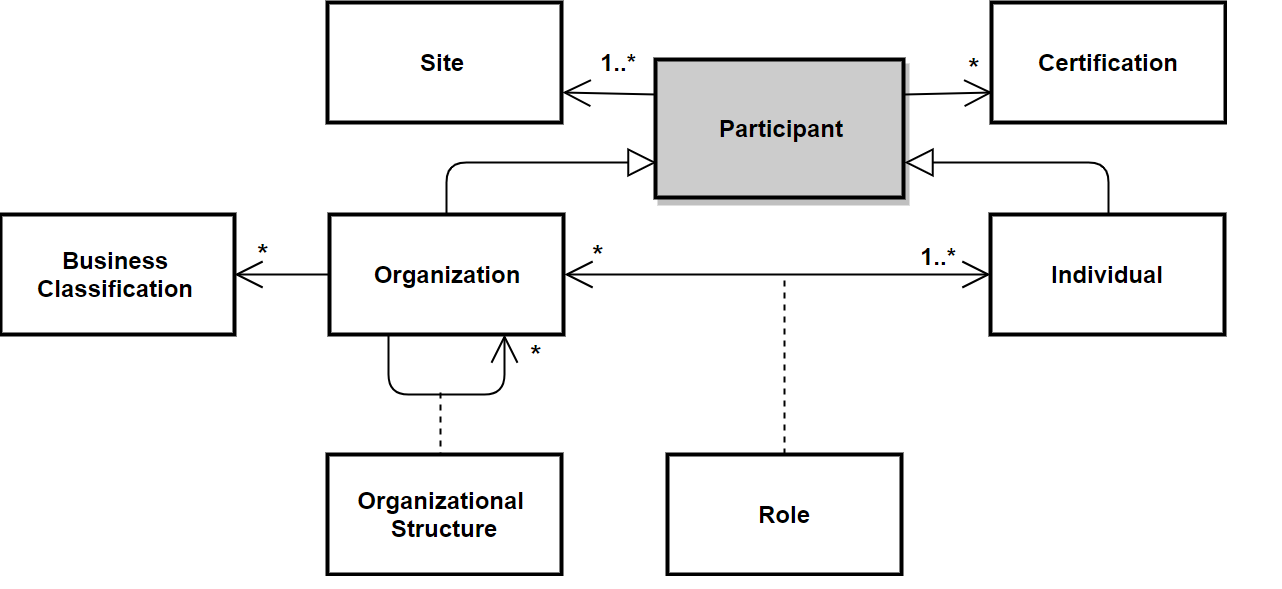
\includegraphics[width=4.68in,height=2.15in]{./media/image49.png}
		\caption{Participant concept (outline)}
		\label{fig:Participant_concept_outline}
	\end{Center}
\end{figure}


%%%%%%%%%%%%%%%%%%%% Figure/Image No: 34 Ends here %%%%%%%%%%%%%%%%%%%%

\subparagraph*{Connector}
%\addcontentsline{toc}{subparagraph}{Connector}
The Connector is the central technological building block of the International Data Spaces. It is a dedicated software component allowing Participants to exchange, share and process digital content. At the same time, the Connector ensures that the data sovereignty of the Data Owner is always guaranteed. Depending on the type of configuration, the Connector’s tamper-proof runtime hosts a variety of system services ensuring, for example, secure bidirectional communication, enforcement of content usage policies, system monitoring, and logging of content transactions for clearing purposes. The functional range of a generic Connector may be extended by custom software (Data Apps), allowing data processing, visualization, persistence etc. 

Roles belonging to the Intermediary category are based on the Connector technology. For example, the Broker Service Provider receives and provides metadata and maintains a metadata registry, the App Store provides Data Apps, and the Vocabulary Hub provides shared vocabularies and related (schema) documents. 

Example: \textit{A Base Connector operated by AAStat at WGS84; coordinates: 50$ ^{\circ} $ 45'44.6"N 7$ ^{\circ} $ 02'01.2"E. It provides a HTTPS 2.0 host serving traffic sensor data. The Connector has limited capabilities only (IoT device) and holds a base certification level}. 

\textbf{DEPLOYMENT CONTEXT }The Deployment Context of a Connector records, among other things, the Connector’s location (e.g. the data center, coordinates), the type of its deployment (on-premises or cloud-based), and the name of the Participant it is operated by (i.e. the Service Provider). Depending on the policy, this information may affect context-based routing of content. 

\textbf{SECURITY PROFILE} The Security Profile indicates the capabilities of a Connector to maintain a controlled, secure and trusted environment for exchanging, sharing and processing digital content in terms of properties (such as remote integrity verification, application isolation, usage control support, etc.). A counterpart in the data exchange may evaluate this information, alongside with the level of Certification, in order to assess the Connector’s technical trustworthiness. 

\textbf{CATALOG} Connectors may expose an arbitrary number of Resources that provide or consume digital content. The Catalog comprises a metadata model of those Resources constructed in accordance with the IDS Vocabulary. Optionally, the Catalog, or individual sets of Resource metadata, may be advertised via intermediary nodes (such as the Broker Service Provider or the App Store Provider).

\textbf{HOST} Each Host represents an individual communication capability of the Connector, a server that exposes Resources via Endpoints (HTTPS URLs, MQTT topics, etc.) according to the communication protocol supported.



%%%%%%%%%%%%%%%%%%%% Figure/Image No: 35 starts here %%%%%%%%%%%%%%%%%%%%

\begin{figure}[H]
	\begin{Center}
		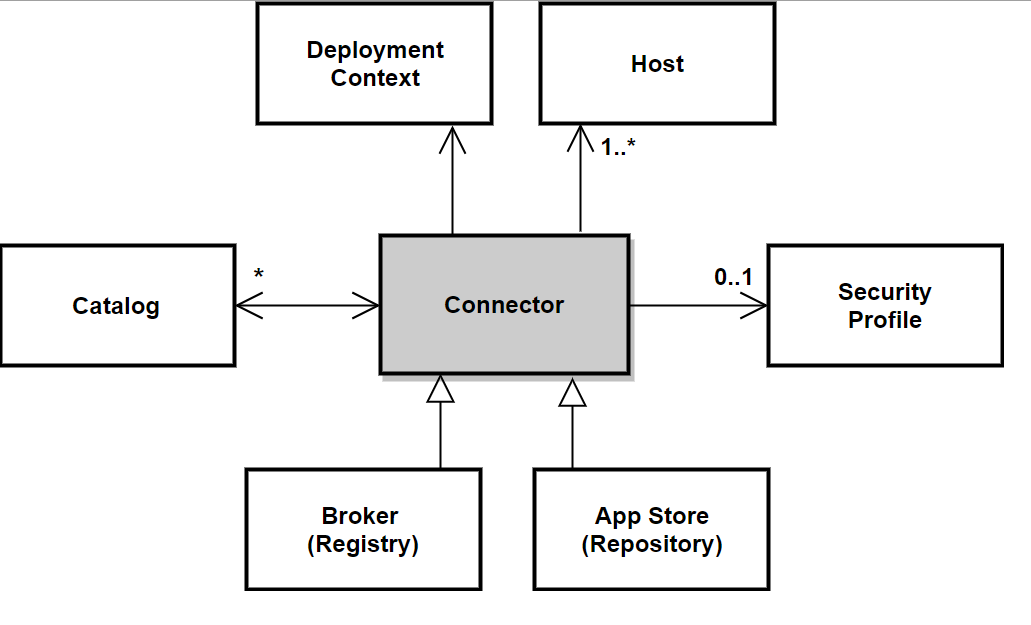
\includegraphics[width=3.92in,height=2.38in]{./media/image50.png}
		\caption{Connector concept (outline)}
		\label{fig:Connector_concept_outline}
	\end{Center}
\end{figure}


%%%%%%%%%%%%%%%%%%%% Figure/Image No: 35 Ends here %%%%%%%%%%%%%%%%%%%%


\subparagraph*{Certification}
%\addcontentsline{toc}{subparagraph}{Certification}
\textit{Certification} aims at determining and formally stating compliance of a Participant or an infrastructure component (basically the Connector) with a predefined set of evaluation criteria. 

Example: \textit{Basic Component Certification based on a self-assessment}.

\textbf{EVALUATION FACILITY }An \textit{Evaluation Facility} carries out the evaluation part during a Participant Certification process, It issues the corresponding Certifications of compliance according to the given \textit{Certification Scheme} (i.e. the processes, roles, evaluation methods, and target criteria). Appointed by the International Data Spaces Association, the \textit{Certification Body }oversees the certification process, defines standardized evaluation procedures, and supervises all activities of the Evaluation Facilities. 

\textbf{CERTIFICATION LEVEL} A successfully completed Certification process results in the assignment of a predefined \textit{Certification Level}, based on a combination of an underlying set of criteria and the depth of the evaluation method chosen. Here, a $``$higher$"$  Certification Level transitively subsumes $``$lower$"$  levels allowing for queries based on a least required level. Certification information is stored in the Participant’s metadata description and attached to the attributes of the X.509 certificate, along with its Validity Period. Certification is expected to be automatically revoked after that date, unless it has been reasserted. 



%%%%%%%%%%%%%%%%%%%% Figure/Image No: 36 starts here %%%%%%%%%%%%%%%%%%%%

\begin{figure}[H]
	\begin{Center}
		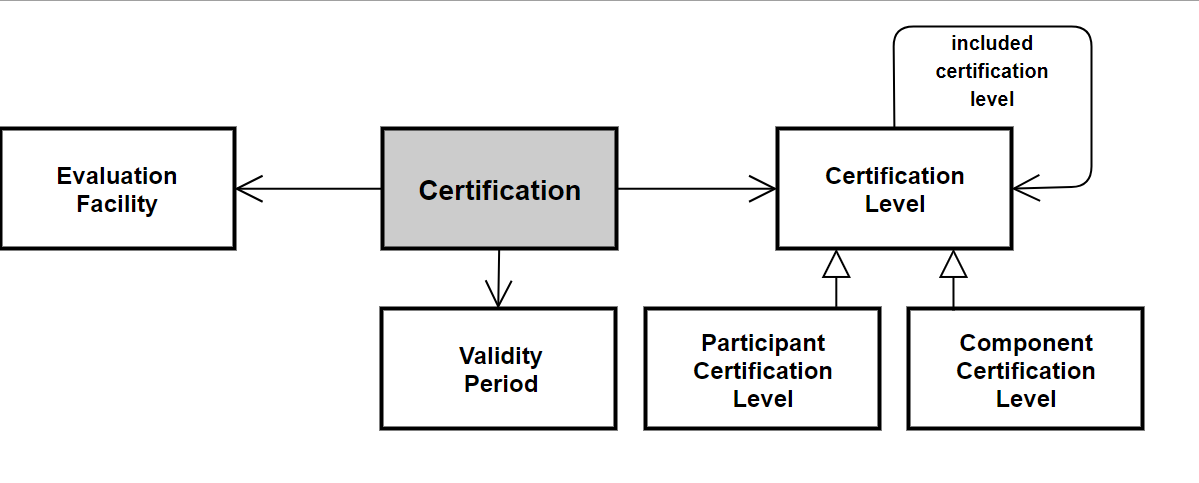
\includegraphics[width=4.5in,height=1.81in]{./media/image51.png}
		\caption{Certification concept (outline)}
		\label{fig:Certification_concept_outline}
	\end{Center}
\end{figure}


%%%%%%%%%%%%%%%%%%%% Figure/Image No: 36 Ends here %%%%%%%%%%%%%%%%%%%%

\subparagraph*{(Usage) Contract}
%\addcontentsline{toc}{subparagraph}{(Usage) Contract}
A Usage Contract formalizes the expectations regarding the behavior of Participants involved in a data exchange transaction in a declarative, technology-agnostic way. It constitutes a unique, binding agreement between the Parties on Resource usage conditions as a result of an (automated) negotiation process. Digital Usage Contracts are to be maintained in a safe, unforgeable manner (e.g. blockchain). They are the foundation for clearing and configuring the Resource’s \textit{access control} policies, and for perpetual evaluation and \textit{enforcement }by Usage Control Frameworks, like MYDATA Control\footnote{https://www.mydata-control.de/ }. 

Example: \textit{Agreement between the Data Consumer YourCargo and Data Provider AAStat valid from 2019/03/01 till 2019/12/31 to provide push notifications about delays and traffic obstructions at some enumerated routes. First 5000 messages are free of charge, the remaining are charged on quantity base (5€/1000 messages).}

\textbf{RESOURCE} Usage Policies originally published alongside with a Resource (Contract Offer) are the starting point of a Contract negotiation process. Over the course of this process, any incomplete or newly agreed details regarding Resource exchange are complemented, such as the identification of the Resource content in question, communication Endpoints, authorization token(s), or the provisioning period. 

\textbf{RULE} Likewise, applicable Rules are selected and configured in accordance with the Data Provider’s demand and the Data Consumer’s economic, legal and technical options. By agreeing on a Usage Contract, the Data Consumer explicitly confirms its capability of implementing and enforcing the stipulated rules.



%%%%%%%%%%%%%%%%%%%% Figure/Image No: 37 starts here %%%%%%%%%%%%%%%%%%%%

\begin{figure}[H]
	\begin{Center}
		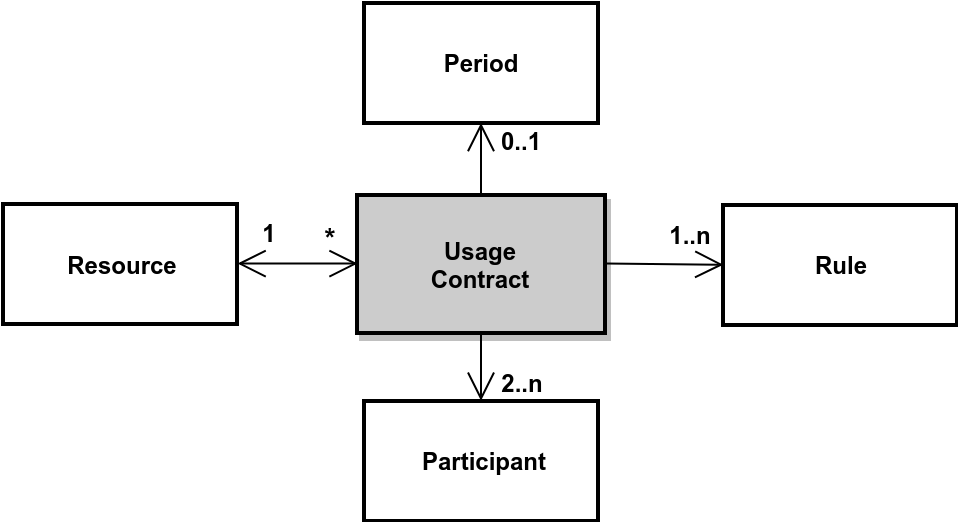
\includegraphics[width=4.67in,height=2.55in]{./media/image52.png}
		\caption{Usage Contract concept (outline)}
		\label{fig:Usage_Contract_concept_outline}
	\end{Center}
\end{figure}


%%%%%%%%%%%%%%%%%%%% Figure/Image No: 37 Ends here %%%%%%%%%%%%%%%%%%%%

\paragraph{Summary\\}
%\addcontentsline{toc}{paragraph}{Summary}
The previous section introduced the Conceptual Representation of the Information Model with the help of the concern hexagon (C-hexagon). Each corner of the hexagon represents a distinguished concern contributing to the concept of the Digital Resource in the context of the International Data Spaces: 

\begin{itemize}
	\item The \textit{Content} concern deals with the description of a Resource’s inherent substance, i.e. its $``$content$"$  available in any machine-interpretable, binary format. 

	\item The \textit{Context} concern deals with temporal and spatial aspects as well as with real-world entities a Resource’s content relates to. 

	\item The \textit{Concept} concern deals with the modeling of the meaning, annotation, and interpretation of entities introduced by another Resource concerns such as Content and Context. 

	\item The \textit{Communication} concern deals with means to communicate a Resource’s content in one of the Representations available. 

	\item The \textit{Commodity }concern helps to assess the value and utility of a Resource. 

	\item The \textit{Community of trust} concern considers the fundamental requirement of the International Data Spaces for exchanging and sharing Resources between a Data Provider and a Data Consumer in a secure and trusted way, while preserving the data sovereignty of the Data Owner.

\end{itemize}

The main aspects covered by the six concerns are summarized in Figure \ref{fig:Detailed_concern_hexagon}.


%%%%%%%%%%%%%%%%%%%% Figure/Image No: 38 starts here %%%%%%%%%%%%%%%%%%%%

\begin{figure}[H]
	\begin{Center}
		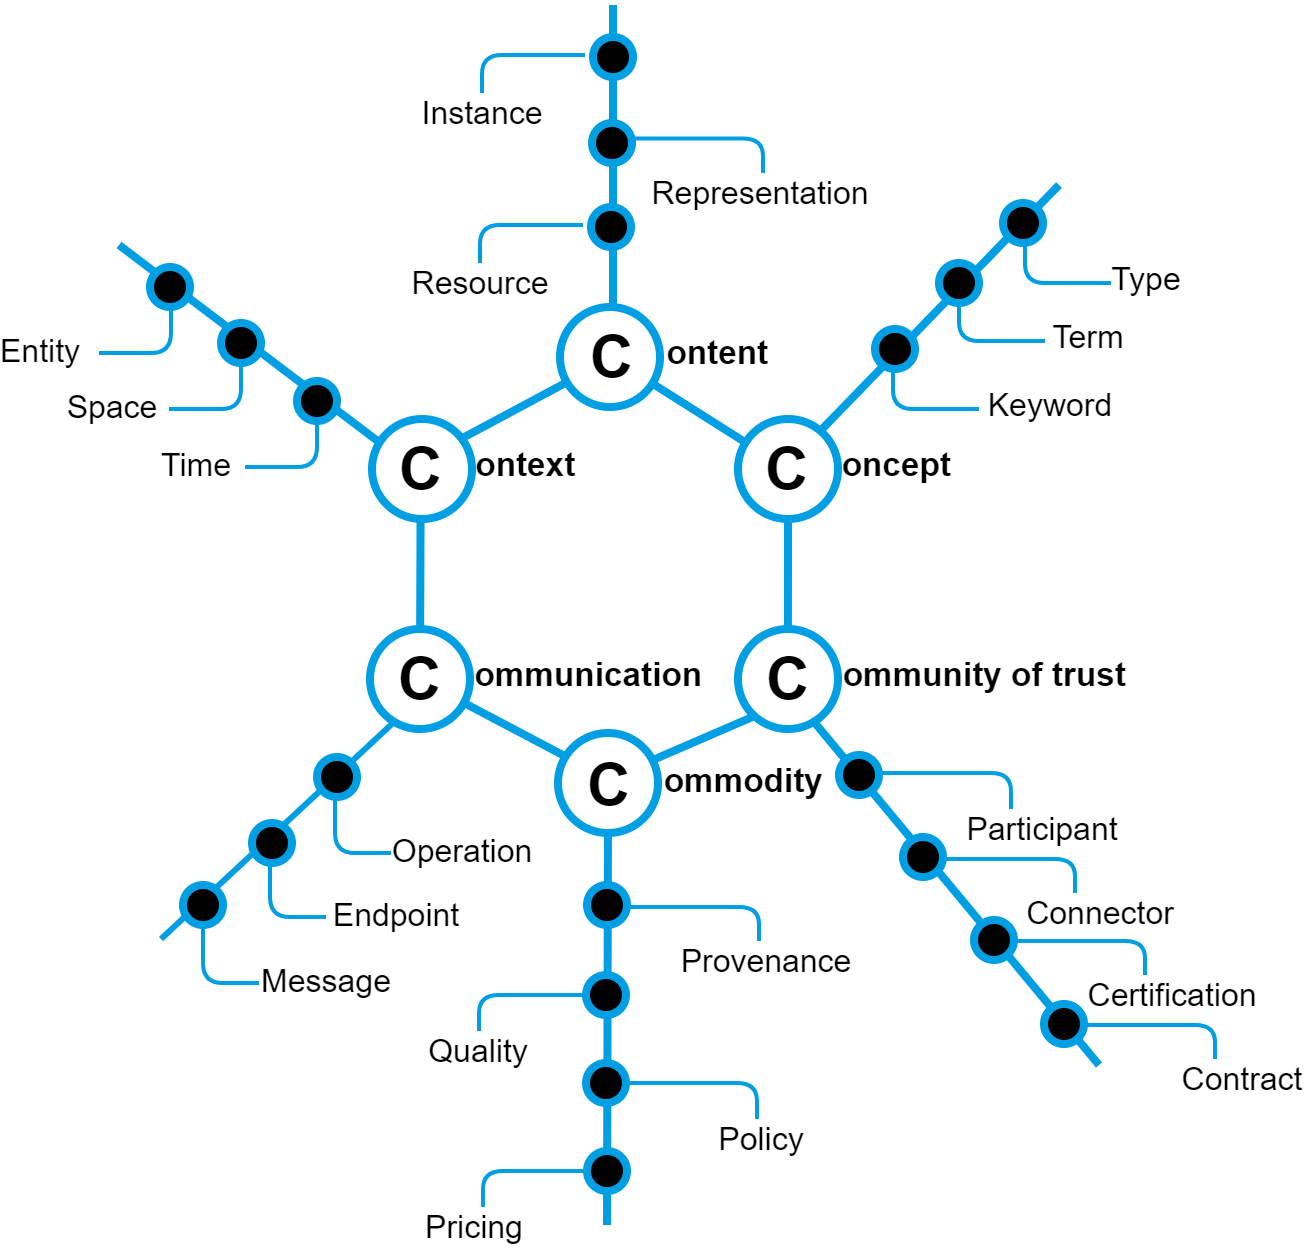
\includegraphics[width=6.53in,height=5.96in]{./media/image53.png}
		\caption{Detailed concern hexagon}
		\label{fig:Detailed_concern_hexagon}
	\end{Center}
\end{figure}


%%%%%%%%%%%%%%%%%%%% Figure/Image No: 38 Ends here %%%%%%%%%%%%%%%%%%%%


\subsubsection{Vocabularies}
%\addcontentsline{toc}{subsubsection}{Vocabularies}
The IDS expresses its Information Model as an RDF ontology in order to provide unambiguous identifiers and formalized definitions of its concepts and relations. To simplify the integration of the IDS ontology, descriptions directly connected to the respective concepts, as well as links to widely-known concepts of so called upper-level ontologies, provide further explanations. As data exchange between different parties is at the core of the IDS, only a fundamental core vocabulary for data descriptions and data exchange invocations is required for all IDS participants. Domain-specific vocabularies may be used wherever necessary to extend the core concepts and to provide more information on data provided or requested.

\subsubsection{Data App Interfaces}
%\addcontentsline{toc}{subsubsection}{Data App Interfaces}
Similar to an IDS Connector providing information on its identity, functional range, and interaction capabilities, an IDS Data App provides information about itself according to the IDS Information Model. A description file contains details about the intended usage and purpose of the Data App, the security level, and the licensing model applied. In addition, a Data Provider may describe a Data App with vocabularies outside the IDS core ontology (for instance, domain specific explanations may require further terms and concepts).

The description of Data Apps facilitates the discovery and selection of a Data App in an IDS App Store. Consequently, metadata must contain all necessary information to specify the value proposition and the applicability of the respective Data App. Furthermore, metadata is a fundamental building block for the deployment and composition of several Data Apps inside an IDS Connector. Therefore, all operations have to be defined in terms of input and output parameters, bound protocols, and endpoints. Preconditions and postconditions need to be made explicit, and effects on the environment must be outlined.
